\documentclass[../main.tex]{subfiles}

\begin{document}

\subsubsection*{Methodology}
\subsubsection*{Data analysis}

    \begin{figure}
        \centering
        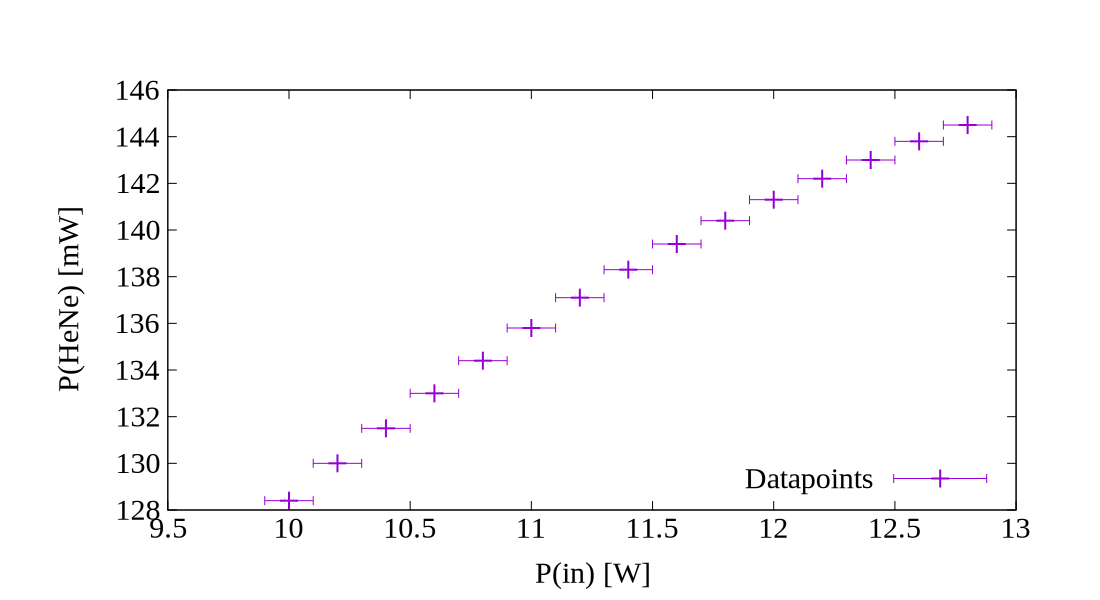
\includegraphics[width=0.8\textwidth]{Bilddateien/2/P(HeNe)overP(in).png}
        \caption{The output power of the HeNe laser as a function of the input power.}
    \end{figure}

    To convert from the initially measured current to the effectively used power we used the voltage $U_{\textit{in}} = (2.0\pm 0.1)\;\si{\kV}$ and the conversion formula $P_{\textit{in}}(I) = I \cdot U_{\textit{in}}$. Because the used measurement tool to capture the current does not provide an uncertainty, we only used the given voltage error for the plots $x$ axis. In the $y$ axis we noted a compareably small error of $\SI{0.1}{\mW}$ during the experiment, which cannot be displayed against the data points. We assume it therefore to be negligible. 

    Because the correct functional relationship between the input and output power is unknown, we used several fitting functions such as sqrt, ln and linear. The best approximation was achieved using ln, so let $f_a(x) := a_1\cdot \ln(a_2\cdot x + a_3) + a_4$ and $a$ be the fitting vector. Then table \ref{tab:fitting_vector_logfit} shows the fitting vector $a$ for the given rescaled dataset. 

    \begin{table}[H]
        \centering
        \begin{tabular}{|c|c|c|c}
            \hline
             & $a_i$ & $u(a_i)$ \\
            \hline\hline
            $a_1$ & $8.60188$ & $9.095$ \\
            $a_2$ & $2.88749$ & $6.693$ \\
            $a_3$ & $-27.5754$ & $62.23$ \\
            $a_4$ & $118.268$ & $5.013$ \\
            \hline
        \end{tabular}
        \caption{The fitting vector $a$ for the function $f_a$. \color{red}TODO: Add units.}
        \label{tab:fitting_vector_logfit}
    \end{table}

    To calulate the minimal input power $P_0$ required to achieve lasing we solve $0 = f_a(P_0)$ and get 




\end{document}